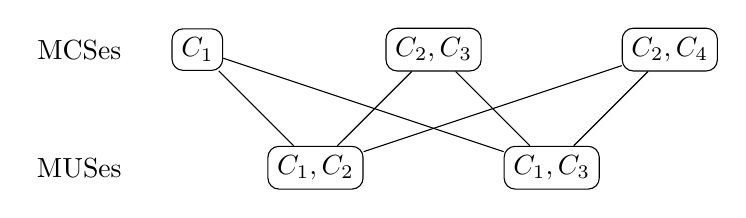
\begin{tikzpicture}[scale=1.5, 
				    state/.style={draw, rounded corners, fill=none,
				    			  text centered, text=black}]
	\node[] (u0) at (1, 2) {MCSes};
	\node[state] (u1) at (2, 2) {$C_{1}$};
	\node[state] (u2) at (4, 2) {$C_{2}, C_{3}$};
	\node[state] (u3) at (6, 2) {$C_{2}, C_{4}$};
	\node[state] (u4) at (3, 1) {$C_{1}, C_{2}$};
	\node[state] (u5) at (5, 1) {$C_{1}, C_{3}$};
	\node[] (u6) at (1, 1) {MUSes};
	
	\path[-] 	(u1)  edge   (u4);
	\path[-] 	(u1)  edge   (u5);
	\path[-] 	(u2)  edge   (u4);
	\path[-] 	(u2)  edge   (u5);
	\path[-] 	(u3)  edge   (u4);
	\path[-] 	(u3)  edge   (u5);

\end{tikzpicture}
